%+----------------------------------------------------------------------------+
%| SLIDES: Longer presentation on my paper 1805.01696
%| Chapter: multisymplectic geometry in hydrodynamics
%| Author: Antonio miti
%| Event: Visit in Salerno, March 2019
%+----------------------------------------------------------------------------+


%- HandOut Flag -----------------------------------------------------------------------------------------
\newif\ifHandout
	\Handouttrue  %uncomment for the printable version

%- D0cum3nt ----------------------------------------------------------------------------------------------
\documentclass[beamer,10pt]{standalone}



%- Packages ----------------------------------------------------------------------------------------------
\usepackage[mode=buildnew,subpreambles=true]{standalone}
\usepackage{amsmath, amssymb,mathtools}
\usepackage{tikz}
\usetikzlibrary{arrows,shapes,calc}
\usetikzlibrary{decorations.pathmorphing}
\usepackage{tikz-cd}
\usepackage{graphicx, animate}
\usepackage{hyperref}
\usepackage[english]{babel}
\usepackage{stackengine}
\usepackage{fourier} %\bomb
%%\usepackage{marvosym} %\Lightning

%--Beamer Style-----------------------------------------------------------------------------------------------
\usetheme{toninus}









%---------------------------------------------------------------------------------------------------------------------------------------------------
%- D0cum3nt ----------------------------------------------------------------------------------------------------------------------------------
\begin{document}
%------------------------------------------------------------------------------------------------


%--------------------------------------------------------------------------------------------------------------------------------
\begin{frame}{An application in hydrodynamics}
	\begin{columns}
		\begin{column}[T]{0.5\textwidth}
	        \centering
	        \resizebox {0.85\columnwidth} {!} {
				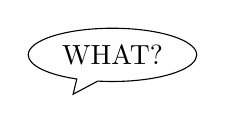
\begin{tikzpicture}
					\node[ellipse callout,draw, callout absolute pointer={(0.5,0)}]   at (1,0.5)
					{WHAT?};
				\end{tikzpicture}
			}
			\begin{block}{Honest Claim}
				\begin{itemize}
					\item Explicit construction of an \alert{Homotopy co-momentum Map}
					\item w.r.t. a pair Lie algebra - MultiSymplectic manifold \\
							relevant to hydrodynamics %~
				\end{itemize}
			\end{block}
		\end{column}
		\begin{column}[T]{0.5\textwidth} 
	        \centering
	        \resizebox {0.85\columnwidth} {!} {
				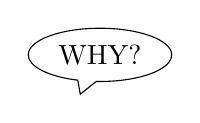
\begin{tikzpicture}
					\node[ellipse callout,draw, callout absolute pointer={(0.75,0)}]   at (1,0.5)					{WHY?};
				\end{tikzpicture}
			}
			\begin{block}{Honest Motivation}
				\begin{itemize}
					\item Provide an application of the Homotopy co-momentum Map machinery
						related to a mechanical problem
				\end{itemize}
			\end{block}		
		\end{column}
		%

	\end{columns}
%	\vspace{2ex}
%	\begin{keywordblock}
%		\begin{tabular}{|c|c|c|}
%			\hline 
%			symplectic & $\rightsquigarrow$ & multisymplectic \\ 
%			\hline 
%			Observables (Poisson) algebra & $\rightsquigarrow$ & Observables $L-\infty$ algebra \\ 
%			\hline 
%			Co-moment map & $\rightsquigarrow$ & Homotopy co-momentum map \\ 
%			\hline 
%		\end{tabular} 
%	\end{keywordblock}
\end{frame}
\note{
			An application in hydrodynamics
}
%---------------------------------------------------------------------------------------------------------------------------------------------------



%---------------------------------------------------------------------------------------------------------------------------------------------------
  \begin{frame}{Hydrodynamical $\mathfrak{g}$- action}
	\begin{columns}[T] % align columns
	\begin{column}{.4\textwidth}
			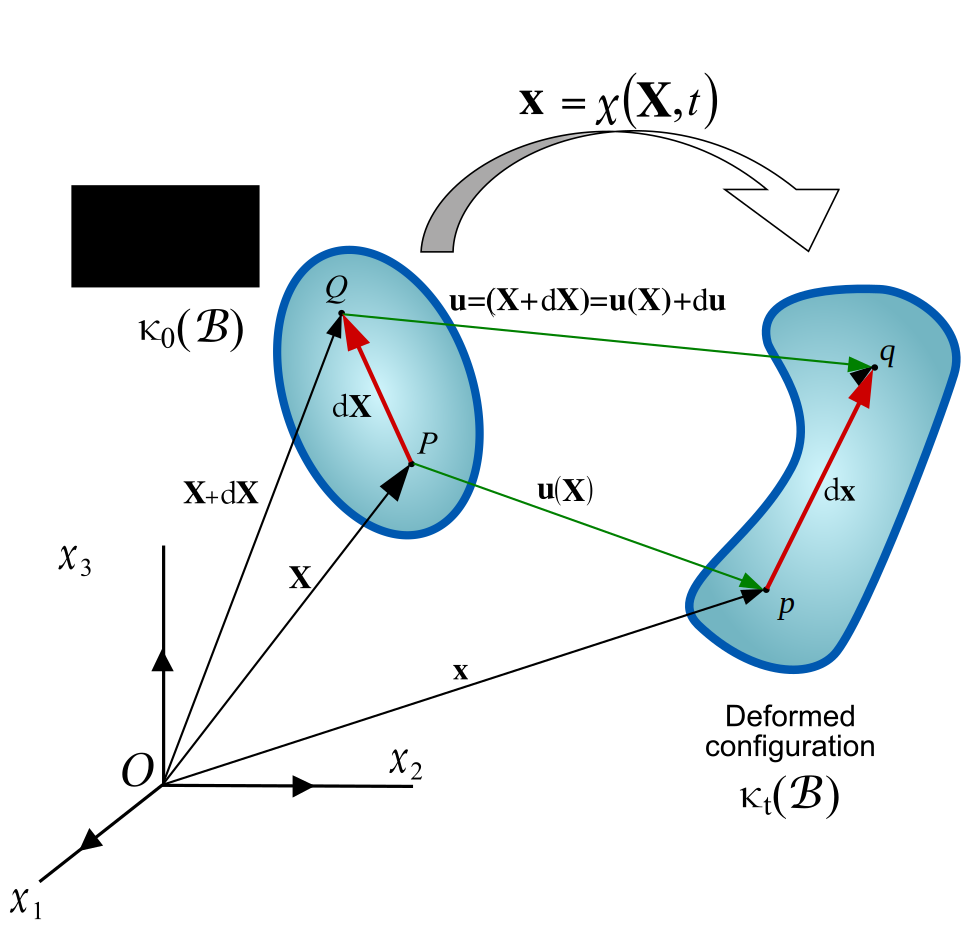
\includegraphics[width=\linewidth]{Pictures/Continuum_body_deformation}
	\end{column}
	%
	\hfill
	%
	\begin{column}{.6\textwidth}
		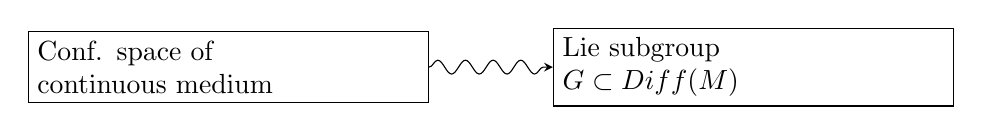
\begin{tikzpicture}[
			text width=0.4\linewidth,
			node distance=0.55\linewidth,
			]
			\node [rectangle,draw] (lhs) {Conf. space of\\ continuous medium};
			\node [rectangle,draw,right of=lhs] (rhs) {Lie subgroup \\$G \subset Diff(M)$};
			\draw[-stealth,decorate,decoration={snake}] (lhs) -- (rhs);
		\end{tikzpicture}

		Examples:
		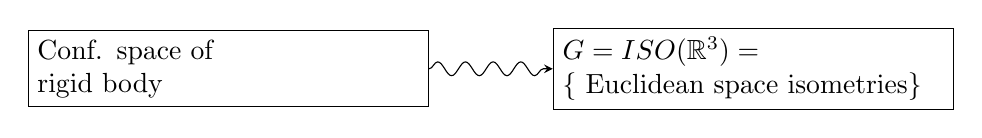
\begin{tikzpicture}[
			text width=0.4\linewidth,
			node distance=0.55\linewidth,
			]
			\node [rectangle,draw] (lhs) {Conf. space of\\ rigid body};
			\node [rectangle,draw,right of=lhs] (rhs) {$G=ISO(\mathbb{R}^3)=$\\ $\{$
				Euclidean space isometries$\}$};
			\draw[-stealth,decorate,decoration={snake}] (lhs) -- (rhs);
		\end{tikzpicture}
		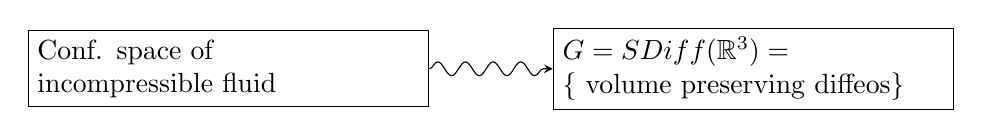
\begin{tikzpicture}[
			text width=0.4\linewidth,
			node distance=0.55\linewidth,
			]
			\node [rectangle,draw] (lhs) {Conf. space of\\ incompressible fluid};
			\node [rectangle,draw,right of=lhs] (rhs) {$G= SDiff(\mathbb{R}^3)=$\\ $\{$
				volume preserving diffeos$\}$};
			\draw[-stealth,decorate,decoration={snake}] (lhs) -- (rhs);
		\end{tikzpicture}
	\end{column}%
	\end{columns}
	\pause
  	\begin{propblock}[$(\mathbb{R}^3,\nu = dx\wedge dy\wedge dz)$ is 2-plectic]
  		\begin{itemize}
  			\item \emph{(Easy proof)} $\quad \iota_v \nu = \frac{1}{2}\epsilon_{i j k} v^i dx^j \wedge dx^k = 0 \; \Leftrightarrow \; v=0 $;
  			\item \emph{(Conceptual proof)} $\quad \alpha^{(1)} = \ast \circ \flat$ is invertible.
  		\end{itemize}
  	\end{propblock}
%		\begin{claimblock} Any oriented manifold is multisymplectic w.r.t. the volume form. \end{claimblock}

		\pause
		 	Consider a subalgebra of the infinitesimal action of $SDiff(\mathbb{R}^3)$:
		  	\begin{displaymath}
		  		\mathfrak{g} = sdiff_0(M) = \lbrace  X \in \mathfrak{X} \quad\vert\quad div X = 0, \textrm{\emph{ rapidly vanishing at }}\infty \rbrace
		  	\end{displaymath}
		  	\centering \alert{(Infinite dimensional Lie algebra!)}
  
  \end{frame}
  \note[itemize]{
	%\item  Now we are ready to get to the real business. Namely, give an explicitly construction of a HCMM related to hydrodynamics.
	\item We are working in the setting of \emph{geometric continuum mechanics} .\\
		Recall that the configuration space of a continuum object is encoded via diffeomorphisms. In the case of an incompressible fluid is encoded via volume-preserving diffeomorphisms.
	\item (Configution space is the set of spatial displacement of a mechanical systems. These are different from the \emph{physical states}.
	\item Such manifolds are infinite dimensional. Particular caution has to be taken when defying in what sense they are smooth.
	\item However, what really pertains to the construction of a moment map is the infinitesimal action, i.e. the Lie algebra. In our case, the infinitesimal action to be considered is via divergence-free vector fields.
	\item (Notation): In the following M will be the 3 dimensional Euclidean Space.
	\item The key, but trivial, observation is that the standard volume form on the euclidean space is a multisymplectic form.
	\item In the following, we will see that the standard Riemannian structure takes a role in our construction. 
	That the reason to show also a "conceptual proof".
	\item Notation: $\ast = $ and $\sharp = $ are respectively the Hodge operator and the Riemmanian sharp operator pertaining to the standard metric in $\mathbb{R}^3$.	
  }
%------------------------------------------------------------------------------------------------


%------------------------------------------------------------------------------------------------
  \subsection{Explicit Construction of the HCMM}
  \begin{frame}{Hydrodynamical homotopy co-momentum map}
  	\begin{claimblock}
  		Explicit construction of an HCMM for $SDiff_0 \circlearrowright (\mathbb{R}^3,\nu)$
  	\end{claimblock}
	\begin{columns}
		\begin{column}[c]{.5\linewidth}
		  	\begin{itemize}
		  		\item The observables are  $$L= \Omega^1_{\textrm{ham}}(\mathbb{R}^3)\oplus\Omega^0(\mathbb{R}^3)$$
		  		\item HCMM consists of a pair of functions:
					\begin{align*}
						f_1 &\colon \mathfrak{g} \rightarrow \Omega^1_{\textrm{ham}}(\mathbb{R}^3) \\
						f_2 &\colon \mathfrak{g}\wedge\mathfrak{g} \rightarrow C^\infty(\mathbb{R}^3)
					\end{align*}	
		  	\end{itemize}
		\end{column}	
	  	\hfill  	
		\begin{column}[c]{.5\linewidth}
  		\includestandalone[width=\textwidth]{Pictures/Figure_Euclid_Trigger}
 	 	\end{column}
 	 \end{columns}
 	\begin{columns}
		\begin{column}[c]{.8\linewidth}
		 	 \begin{itemize}
				\item Satisfying the following system:
					\begin{displaymath}
						\begin{cases}
							\textrm{d} f_1(\xi) = \iota_\xi \nu = -\alpha^1(\xi) \\
							\textrm{d} f_2(\xi_1 \wedge \xi_2) = f_1\left([\xi_1,\xi_2]\right) - \iota_{\xi_2}\iota_{\xi_1} \nu 
							 := \mu_2(\xi_1,\xi_2)\\
							f_2\left(\partial \xi_1 \wedge \xi_2 \wedge \xi_3 \right) = \iota_{\xi_3}\iota_{\xi_2}\iota_{\xi_1} \nu
						\end{cases}
					\end{displaymath}
		 	 \end{itemize}
 	 	\end{column}
		\begin{column}[c]{.2\linewidth}
 	 	\end{column}
 	 \end{columns}
  \end{frame}
	\note[itemize]{
		\item (Regarding the diagram)
		\item On the left there is the part of the Chevalley-Eilemberg complex that interact with the L-$\infty$ algebra of observables.
		\item On the right there is the whole de Rham complex of the manifold $M=\mathbb{R}^3$.
		\item Even if only $\Omega^1$ and $\Omega^0$ take part in the definition of a $HCMM$, the Riemmanian structure determine a correspondence with the rest of the de Rham complex.
		\item In order to give an HCMM for this action is necessary to give a solution of the system of 3 equations below.
		\item Recall: $ 	\ast: \Omega^k \rightarrow \Omega^{n-k}$ where $\ast \sigma$ is defined as the unique form such
		 that $ \omega \wedge \ast \sigma = \nu \lbrace \omega, \sigma \rbrace$ where 
		 $\langle,\rangle$ is the inner product on forms induced by the metric. 
	}  
%---------------------------------------------------------------------------------------------------------------------------------------------------


%--------------------------------------------------------------------------------------------------------------------------------------------------- 
  \begin{frame}[t]{Explicit Construction of the HCMM}
		\begin{enumerate}
			\item<1-> Fix $\vec{b} \in \mathfrak{g}$ and define $f_1(b) := -\vec{A}^\flat$.\\ 
				The first equation is equivalent to solve
				\begin{displaymath}
					\tag{equation of magnetostatic}
					{\rm curl}(\vec{A})=\vec{b}
				\end{displaymath}
				This equation admits a solution 
				\begin{displaymath}
					\tag{Biot-Savart law}
					\vec{A}(r) = \int\frac{\vec{b}\times(\vec{r}-\vec{r}')}{|\vec{r}-\vec{r}'|^3}\textrm{d}r'
				\end{displaymath}							
				\alert {Defined up to a gradient \emph{(gauge freedom)}}. 
			%
			\item<2-> $\mu_2(\xi_1,\xi_2)$ is closed $\forall \xi\in\mathfrak{g}$ $\xRightarrow[\text{lemma}]{\text{Poincar\'e}}$ is exact.\\
				%Hence it is also exact \emph{(Poincar\'e lemma)}.\\
				Take as $f_2(\xi_1,\xi_2)$ a primitive $0$-form, \alert{determined up to a constant $c(\xi_1,\xi_2)$}.
			%
			\item<3-> Third equation is a priori only true up to a constant $c(\xi_1, \xi_2, \xi_3)$.\\
				The constant is zero since $\nu(\xi_1, \xi_2, \xi_3)$ vanishes at infinity and 
				the same is true for $f_2(\partial q)$ upon solving the related Poisson equation
 				\begin{displaymath}
 			 		\Delta f_2(\partial q) = \Delta \nu(\xi_1, \xi_2, \xi_3)			
 				\end{displaymath}
		\end{enumerate}
  \end{frame}
  \note[enumerate]{
  	\item	
  		\begin{itemize}
		  	\item Exploiting the correspondence between tangent fields and 1-form given by the metric is possible to recast the first equation in a simple vector calculus equation containing  the curl.
		  	\item Such equation is the well-known equation of magnetostatic with admits solution by the Biot-Savart law.
		  	\item In the context of hydrodynamic $A$ can be interpreted as a \emph{velocity field} and $b$ as the corresponding vorticity. (See slide for further details)  		
  		\end{itemize}
  	\item In the language of physics, such primitive form is often called "a potential".
  	\item 
  		\begin{itemize}
  			\item (Notation) $q = \xi_1 \wedge \xi_2 \wedge x_3$.
  			\item Last equation tells us that $f_2(\partial q)$ and $ \nu(q)$ differs by a constant. But since both of them vanish at infinity this constant has to be zero.
  			\item The condition of vanishing at infinity has been imposed in order to fulfil the last equation.
  		\end{itemize}
  	\item[$\triangleright$] This construction can be generalized to oriented Riemannian manifolds with further cohomological condition. 
  		See appendix, pag: \ref{frame:RiemannianGeneralization}.
  }
%---------------------------------------------------------------------------------------------------------------------------------------------------


%---------------------------------------------------------------------------------------------------------------------------------------------------
\subsection{Hydrodynamics interpretation}
\begin{frame}[fragile]{Hydrodynamics interpretation}
		Consider the loop spaces $L{\mathbb R}^3$,\\
		%
		\begin{propblock}[HCMM for $G\circlearrowright(\mathbb{R}^3,\nu)$ induces \\an ordinary co-mo.map for $G\circlearrowright (LS,\nu^{\ell})$]
			The HCMM $f \colon \mathfrak{g} \to L_{\infty}(\mathbb{R}^3,\nu)$ previously given
			\emph{transgresses}	 to
			\begin{displaymath}%\tag{Arnol'd-Marsden-Weinstein\\ hydrodynamical co-momentum map}
				\begin{tikzcd}[column sep= small,row sep=0ex]
					\lambda \colon& \mathfrak{g}	\arrow[r]& C^\infty(LS) \\
					& {\mathbf b}	\arrow[r, mapsto]& \displaystyle \lambda_b(\textvisiblespace) =-\oint_{\textvisiblespace} A^\flat = - \oint_{\textvisiblespace} f_1({\mathbf b}) 
					%	\quad \forall \gamma \in LS		
				\end{tikzcd}	
			\end{displaymath}
			that is a  moment map for the induced action $G$ on the pre-symplectic loop space $(LM,\nu^{\ell})$. (Smooth space in the sense of Brylinski)
		\end{propblock}
		\begin{itemize}
			\item $\lambda$ corresponds to \emph{Arnol'd-Marsden-Weinstein hydrodynamical co-momentum map}  defined on $\infty$-dim. manifolds.
			\item<2-> $\Lambda = \left\lbrace \lambda_{\mathbf b} \right\rbrace_{{\mathbf b}\in\mathfrak{g}}$ is, up to sign, the {\it Rasetti-Regge current algebra}
			\item<3-> There is a naturally defined {\it Poisson brackets} on $\Lambda$:
				\begin{displaymath}
					\{ f_1({\mathbf b}), f_1({\mathbf c}) \} (\cdot):= \iota_{\mathbf c} \iota_{\mathbf b} \nu (\cdot)=
						\nu({\mathbf b}, {\mathbf c}, \cdot) = f_1([{\mathbf b},{\mathbf c}])
					-df_2 ({\mathbf b} \wedge {\mathbf c})
				\end{displaymath}
				\centering\footnotesize(Note: $\lambda$ is (infinitesimally) $G$-equivariant, i.e. $	\{\lambda_{\mathbf b}, \lambda_{\mathbf c} \} = \lambda_{[{\mathbf b}, {\mathbf c}]}$)
		\end{itemize}

    
\end{frame}
\note[itemize]{
  	\item[ ] \textbf{How all of this is relevant in Hydrodynamics?}
  	\item The loop space is the manifold, in the sense of Brylinsky, consisting of all smooth loops in ${\mathbb R}^3$.
  	\item Transgression can be seen as a pull-back along the evaluation map 
  		$${\rm ev}: L{\mathbb R}^3 \times {\mathbb R} \ni (\gamma, t) \mapsto \gamma(t) \in {\mathbb R}^3$$
  		  	For further details see appendix, pag: \ref{frame:LoopSpacesTransgression}.
  	\item Note that the (RR) current pertaining to ${\mathbf b} \in {\mathfrak g}$  is independent of the choice of $B$.
  			See appendix, pag: \ref{frame:RRcurrents} for other informations on this concept or \cite{Rasetti1975},\cite{Penna1992} for a deeper account.
  	\item In \cite{Callies2016} is proved a general result asserting that, roughly speaking,
			homotopy co-momentum maps transgress to homotopy co-momentum maps on loop (and even mapping) spaces. Further details in appendix, pag: \ref{frame:TransgressionHCMM}.
	\item Actually, the ansatz for $f_1$ term in the previous construction has been precisely motivated by this phenomenon. 
}
%------------------------------------------------------------------------------------------------

%------------------------------------------------------------------------------------------------
\begin{frame}{Non Equivariance} 
	%
 	\begin{columns}
		\begin{column}[c]{.5\linewidth}	
			\begin{defblock}[$G$-equivariant HCMM]
				$f_i\colon \Lambda^i\mathfrak g\to \Omega^{n-i}(M)$ \\ 
				Ad(G)-equivariant $ \forall i\in\{1,...,n\}$.
			\end{defblock}		
		\end{column}
		\begin{column}[c]{.5\linewidth}	
			\begin{defblock}[$\mathfrak{g}$-equivariant HCMM]
				$\mathcal{L}_{v_x}(f_i(q))=f_i([x,q])$ \\
				\phantom{\hspace{2cm}}$\forall q\in \Lambda^{i}\mathfrak g , \: x\in \mathfrak g$\\
				\footnotesize{Where $[x,\cdot]$ is $ad(x)$ acting  on $\Lambda^\bullet \mathfrak g$}
				%$f_i\colon \Lambda^i\mathfrak g\to \Omega^{n-i}(M)$
			\end{defblock}		
		\end{column}
	\end{columns}
	\pause
	\vfill
	\begin{propblock}[$(f)$ is not $\mathfrak{g}$-equivariant]
		\underline{Proof:} 
		\footnotesize
		Consider in particular $\xi = \vec{b} \in \mathfrak{g}$, one should check 
		\begin{displaymath}
			\begin{split}
				0 = f_1\left( [\xi, \vec{b}] \right)
				\stackrel{?}{=}
				%=?=
				{\mathcal L}_{\xi} f_1({\vec{b}})  = -{\mathcal L}_{\xi} \vec{A}^\flat &=
					- d \iota_\xi \vec{A}^\flat = - d \langle \vec{A}, \vec{b} \rangle_g
				\qquad \forall \xi \in \mathfrak{g} \\
						\text{(vanishing at infinity condition)} &\Rightarrow \langle \vec{A}, \vec{b} \rangle_g = 0
			\end{split}
%		\begin{split}
%					f_1\left( [\xi, \vec{b}] \right) &= 0 \\
%					 ( \forall \xi\in \mathfrak{g}) \quad \parallel ? & \qquad\\
%					{\mathcal L}_{\xi} f_1({\vec{b}})  &= -{\mathcal L}_{\xi} \vec{A}^\flat =
%					- d \iota_\xi \vec{A}^\flat = - d \langle \vec{A}, \vec{b} \rangle_g
%		\end{split}		
		\end{displaymath}
		%
	 	\begin{columns}
			\begin{column}[c]{.7\linewidth}
				(By contradiction), consider $\vec{b}\in\mathfrak{g}$ supported on two linked flux tubes
				$(\text{supp}(\vec{b}) = \Gamma_1 \cup \Gamma_2)$, one gets
		\begin{displaymath}
			\int \langle \vec{A}, \vec{b} \rangle_g = 2 \mathbf{n} \Phi_1 \Phi_2 
			\qquad \text{with} \quad 
			\Phi_i = \int_{S_i} \hat{n} \cdot \vec{b}\, d\sigma
		\end{displaymath}
		where $n \in \mathbb{N}$ \emph{(Gauss linking number)}, results
		$$\mathbf{n} \neq 0 \qquad \Rightarrow \quad {\mathcal L}_{\xi} f_1({\vec{b}}) \neq 0  \quad \Rightarrow \quad\text{\bomb}$$ 
			\end{column}
			\begin{column}[c]{.45\linewidth}	
				\includegraphics[width=0.9\linewidth]{Pictures/VortexLink}
			\end{column}
		\end{columns}	
	\end{propblock}

		
\end{frame}
\note[itemize]{
    \item We may also naturally ask the question whether the above map $(f)$ is (infinitesimally) {\it G-equivariant}, in the sense of \cite{RWZ}.
    \item In the symplectic case, $G$ connected implies $G$-equivariance. This does not hold true in the multisymplectic case. (ask Leyli!)
    \item In the proof, if $\vec{A}$ is the velocity field of the fluid, $\vec{b}$ is the associated vorticity, the quantity $\langle \vec{A}, \vec{b} \rangle_g$ is called \emph{Helicity}, see below (pag. \ref{Frame:VortexLinks}) for further details.
    \item The proof is by contradiction by exhibiting an example of solenoidal field $\vec{b} = \text{curl}(\vec{A})$ with non vanishing helicity, i.e. not satisfying the condition.\\
    Namely, consider a solenoidal field compactly supported  on a domain $D$ consisting in two disjoint, unknotted but linked closed tubes.
    \item  See \cite{Moffatt-Ricca92} for further elucidation on the non vanishing of the Helicity in the cosidered case.
    Notice that the argument does not depend on the choice of	$\vec{A}$ pertaining to the fixed $\vec{b}$.
    \item The lack of $G$-equivariance is not surprising, since our construction involves Riemannian geometric features.	
}
%------------------------------------------------------------------------------------------------

\end{document}
%-------------------------------------------------------------------------------------------------------------------------------------
\begin{frame}{going beyond fluid}
	\begin{columns}
		\begin{column}[T]{0.5\textwidth}
	        \centering
	        \resizebox {0.85\columnwidth} {!} {
				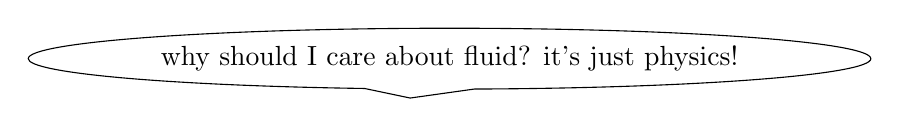
\begin{tikzpicture}
					\node[ellipse callout,draw, callout absolute pointer={(0.5,0)}]   at (1,0.5)
					{why should I care about fluid? it's just physics!};
				\end{tikzpicture}
			}
		\end{column}
		\begin{column}[T]{0.5\textwidth} 
	        \centering
	        \resizebox {0.85\columnwidth} {!} {
				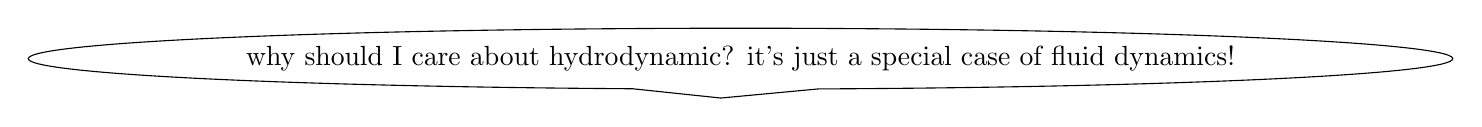
\begin{tikzpicture}
					\node[ellipse callout,draw, callout absolute pointer={(0.75,0)}]   at (1,0.5)					{why should I care about hydrodynamic? it's just a special case of fluid dynamics!};
				\end{tikzpicture}
			}
		\end{column}
	\end{columns}
	\begin{figure}
		\includegraphics[scale=0.5]{Pictures/purity}
	\end{figure}

  	Comic:
  		mathematician: "why should I care about fluid? it's just physics!\\
  		physicists: "why should I care about hydrodynamic? it's just a special case of fluid dynamics!\\  
  		
  	Concetto filosofico / crackpot:\\
  	Così come si usano le geodetiche per sondare le varietà riemmaniane si può usare il fluido perfetto (esteso in tutta la varietà).\\
  	+++ (vedi talk Spera) si può codificare questo problema comunque come una geodetica!
  	
  	Inoltre:\\
  	Ubiquitus role of the group of orientation preserving diffeomorphisms!
\end{frame}
\note[itemize]{
	\item It's a joke from the point of view of theoretician! It's clear that if you are inclined to application there are endless possibilities!

\url{https://xkcd.com/435/}
}
%-------------------------------------------------------------------------------------------------------------------------------------
  